% vim:set textwidth=100:
% vim:set fo+=t:

\documentclass[12pt]{article}

\usepackage{amsmath}
\usepackage[nofiglist,notablist]{endfloat}
\usepackage[usenames,dvipsnames]{color}
\usepackage{color}
\usepackage{authblk}
\usepackage{graphicx}
\usepackage{palatino}
\usepackage[activate={true,nocompatibility},final]{microtype}
\usepackage[super,sort&compress]{natbib}
\pagenumbering{arabic}
\parskip = 0.08in \parindent = 0.0in

% Custom macros for author comments
\newcommand{\Alberto}[1]{\color{ForestGreen}#1\normalcolor }
\newcommand{\Justin}[1]{\color{blue}#1\normalcolor}
\newcommand{\Arijit}[1]{\color{yellow}#1\normalcolor}
\newcommand{\Ken}[1]{\color{red}#1\normalcolor}

\author{Arijit~Roy}
\author{Justin~L.~MacCallum}
\author{Alberto~Perez}
\author{Ken~A.~Dill}
\affil{Laufer Center for Physical and Quantitative Biology\\
    Stony Brook University\\
    Stony Brook, NY 11794-5252.}

\title{Physics-based protein structure prediction and design using the confinement method}

\begin{document}

\maketitle

\begin{abstract}

The calculation of free energy differences is of central importance in the simulation of biochemical
systems. It is particularly difficult to calculate between pairs of macromolecular
conformations as well as a computationally expensive task with existing
methods. In this work, the confinement approach is used to calculate absolute
free energies of biomolecular systems. The method provides two main advantages: it does not require a reaction coordinate or
transition path and it is fast to compute. The free energy calculated can be decomposed into a per
residue contribution in an 
approximate way. Per residue free energy allows us
to identify the reason behind conformational preferences in biomolecules. Through out the article we show its use in different
challenging modeling problems. In particular, we show its use in predicting the conformational
preference of chamaleon sequences (sequences with high sequence identity and different
folds). This sequence dependent conformational preferences and per residue free energy decomposition set the stage for the use of this 
method in protein design. 

\end{abstract}


\section{Introduction}

In computational structural biology there are numerous cases where the free energy difference
between two well defined 
states plays an important role. Examples range from small to large conformational changes of proteins due to
ligand binding, change of pH or other conditions \cite{Meirovitch2007}, \cite{Chipot2007}, \cite{Jorgensen2004}. 
Free energy also plays an important role in the case of protein
folding. The ground breaking work of Christian B. Anfinsen and coworkers showed that the native
structures of small globular proteins have a unique, thermodynamically stable native structure with
their conformation at the global free energy minimum \cite{Anfinsen1973}. Regardless of the starting
point or even after unfolding 
it by changing different condition most proteins will go back to the native state after
reinstituting native like conditions. Often, the changes in free energy between different
conformations is small, but nonetheless crucial in favoring the native state
 since defects in protein folding may be
the molecular cause of a range of human genetic disorders. For example a misfolded protein known as
a
prion can misfold correctly folded proteins when entering a healthy organism.
\Alberto{I'm not sure I understand this here} \Arijit{Thus, Free energy can also act as a scale to identify between the misfolded and the native state of
the protein.} These facts further give free energy a special importance in structural biology.

However, the theoretical calculation of conformational free energy change becomes difficult if the
states of interest are very different \cite{Meirovitch2007}. In such scenario timescales involved in
such conformational transitions may
be beyond the sampling ability of classical molecular dynamics simulation.  Generally, in order to
calculate the free energy a pathway or reaction coordinate is needed with several intermediate structures.
Methods like umbrella sampling \cite{Torrie1977}, thermodynamic integration \cite{Tironi1994} along with classical MD can suffer from
overlap problem and require a large computational effort. The idea of a reaction coordinate became
even more
complicated in the case of protein folding.  As the free energy landscape for protein folding 
is rough \cite{Dill1997}, \cite{Dill2008}, the molecule 
can get trapped in an energy well during conformational sampling. Even with 
advanced methods like replica exchange molecular dynamics, the three dimensional structure may be
trapped in a local minima for a considerable time, giving rise to nonconverged distributions where
misfolded states might be selected as native like
% (give the example of human pin1ww domain from Benout Roux and Klaus Schultan).


The calculation of free energy has been successfully attempted by a number of groups \cite{Meirovitch2007}, 
\cite{Ytreberg2006} - \cite{Zheng2008}. In recent years methods like the Reference system method \cite{Ytreberg2006}, 
Decativated Morphing \cite{Park2008}, Orthogonal Space Random Work \cite{Zheng2008} or the Confinement 
Method \cite{Tyka2006}, \cite{Cecchini2009} to name a few have been used to calculate free energy
differences.
In this work we have applied the confinement method which was originally devoled by Tyka et. al. \cite{Tyka2006} and
Cecchini et. al. \cite{Cecchini2009}. This method relies on the fact that the free energy difference is a state function and 
thus it is independent of the sampling path. This approach uses a thermodynamic cycle where first, non-harmonic degrees of
freedom are removed by applying a series of restraints to the system. Then the free energy of the
remaining harmonic system is obtained using a normal mode calculation and combined with the
non-harmonic part to give the total absolute free energy.  Previously, this method was applied to
calculate the conformational free energy of a 16 amino acid residue peptide, known as BHP.  We have
first reproduced that known result. Then we have applied this method to larger proteins for the
first time. The free energy difference of pairs of conformations in proteins with similar sequence but completely
different fold was calculated. \Alberto{i made this part too long, have to summarize here and define
better inside text?-->} Encouraged by the result, we applied the method to help tackle the
problem of protein conformation ranking. We did this by selecting different targets from the
Critical Assessment of Structure Prediction (CASP) event. In this event, different research groups
try to find the 3D structure of a protein given a sequence in a blind way using their methodologies. Upon comparing
with the real structure it is often seen that several groups are able to generate better structures
than the ones they submit, but are not able to identify them. This is known as the ranking problem,
and this method is able to correctly rank structures in the majority of cases we have tried.
 Finally, we have been exploring the ability of working on a per residue basis to identify which
 residues are the major players in the stabilization/destabilization of a pair of conformations. Our
 initial experience makes us thinkg that this method might be helpful in identifying key residues
 for protein design.

%of protein can be obtained to atomic resolution by X-ray crystallography or NMR. Unfortunately, the
%sheer amount of time and economic investment for structure determination cannot keep up with the
%rate at which proteins of unknown structure are sequenced. Therefore, computational models can be a
%good way to bridge the increasing gap between sequence and structure. In this respect CASP
%(Critical Assessment of Structure Prediction) has played a crucial role which is a community wide
%experiments for the protein structure prediction.



\section{Results and Discussion}

\subsection{The confinement method produces correct results in control experiments}

\Alberto{ This is benchmarking, good internal, but not relevant. Should go to SI,out, or summarized
    in one sentence:  "After reproducing the results of Cecchini and coworkers we were interested in
the ability to apply this method to larger systems"}

\Alberto{As a first step, we performed several control experiments to verify that our implementation of the
confinement method produces results compatible with previous calculations reported in the
literature.

The method has previously been applied to a 16 amino acid residue $\beta$-hairpin from
protein G, known as BHP \cite{Cecchini2009}. We calculated the free energy difference between two different
conformations of the peptide: (1) the native conformation, called bhp1, with a two-stranded
$\beta$-sheet; and (2) a conformation, called bhp3, which has a three-stranded $\beta$-sheet.
Analysis of long (4 $\mu$s) equilibrium simulations \cite{Cecchini2009},\cite{Krivov2004}  shows that bhp1 is the more favorable
configuration by 1.8 kcal/mol. Using the confinement method, we obtain a value 1.7 kcal/mol, which
is in good agreement with the equilibrium simulations and with previous calculations using the
confinement method \cite{Cecchini2009} (see Supporting Information for further details).}

Previous applications of the confiment method have focused on relatively short peptides, up to $17$
residues in length. In this work we apply the confinement method to
larger proteins. On that direction, we first test the confinement method for a chamelon sequence and 
found that it can correctly pick out the prefential structure of the chamelon sequence. Other 
applications we explore in the present work is the re-scoring, or
metaprediction, of structures submitted during the Critical Assessment of Structure Prediction
(CASP) experiment (described in detail later). We computed the relative free energies of predictions
submitted during CASP9, with the expectation that the most native-like prediction will have
the lowest free energy. As a control, for several targets we also calculated the relative free
energy of the experimentally determined structure. \Alberto{should not start with results yet, first
we are describing what we are going to show them} As
Table~\ref{table:casp_control} shows, in most cases, the confinement method correctly assigns a
lower free energy to the experimentally determined structure than to any of the decoys. 
Most interestingly, we decomposed the free energy into its per residue component, which help 
us to identify the residues which stabilize or destabilize a particular conformation of the protein.
%Although differentiating between experimentally determined structures and computer generated predictions is
%not a stringent test of a scoring method---for example, examining the residue-residue packing can
%easily distinguish between the two [ref Rosetta Holes]---the results none the less serve as a useful
%"sanity check".

\begin{table}
\begin{center}
\caption{The confinement method assigns a more favorable free energy to the experimentally
determined structure than to computer-generated predictions. For each target, we examined as many as
five predictions submitted by CASP participants. Positive $\Delta\Delta G$ values indicate that the
experimental structure is predicted to be more favorable than any of the decoys.}
\label{table:casp_control}
\begin{tabular}{l l l}\hline
    CASP Target  & PDB Identifier & $\Delta\Delta G_{native \to best decoy}$ (kcal/mol) \\ \hline
     T0531       &    2KJX        &          $11.15 \pm 0.70$ \\ \hline
     T0538       &    2L09        &          $-3.00 \pm 0.47$ \\ \hline
     T0540       &    3MX7        &          $16.94 \pm 0.49$ \\ \hline
     T0559       &    2L01        &          $2.10 \pm 0.24$ \\ \hline
     T0560       &    2L02        &          $18.00 \pm 0.49$ \\ \hline
     T0569       &    2KWY        &          $20.01 \pm 0.69$  \\ \hline
\end{tabular}
\end{center}

\end{table}


\subsection{The confinement method correctly predicts the structural preferences of chameleon
sequences}

In general, proteins with similar sequences tend to have similar structures. This idea is the basis
of comparative modeling and fold recognition in protein structure prediction. There are, however,
examples---often referred to as chameleon sequences---of proteins with similar sequences that have
remarkably different structures. Orban and co-workers have designed a sequence of 56-residues that
is marginally stable in one of two possible folds. By mutating key residues in this sequence they
are able to stabilize one fold or the other (see Figure~\ref{fig:orban}). Sequences that adopt a mixed alpha/beta structure similar to Protein G
are denoted as ``GB'', while sequences that form a three-helix bundle are denoted as ``GA''. One
pair of sequences (GA88/GB88) are 88 percent identical in sequence and differ in seven positions. Another pair
(GA95/GB95) are 95 percent identical and differ in three positions. The last pair (GA98/GB98) differ
only in a single tyrosine to alanine mutation.

The fact such small changes in sequence can lead to such dramatic changes in structure is rather
remarkable. Accurately predicting the structural preferences of these structures presents a serious
challenge for computational methods \cite{Alexander2007}$-$\cite{Shortle20009}.

We initially approached this problem by making a model of each sequence with the same backbone
structure as its partner chameleon sequence. For example, we took the sequence of GA88 and built a
model with the same overall structure as GB88. We then used the confinement method to assess the
free energy difference between the experimentally determined structure of GA88 and the model (with
the GA88 sequence and the GB88 structure). The confinement method was able to predict the
conformational preferences correctly for all six sequences (data not shown). This is however not
surprising. It is well known [CITE] that it is easy to distinguish computational models from native
structures. Despite the fact that this models are built by having a huge amount of structural
information, it might be possible that we were able to make correct predictions simply
because artefacts of our modeling procedure always lead to the model having a higher free energy
than the experimental structure. 

To avoid this potential problem, we instead computed the relative free energy of two different
structural models for each sequence. One model is based on the GA structure and the other on the GB
structure (see Supporting Information for details on the modeling procedure). This is a much more
realistic test of the confinement method's ability to accurately calculate relative free energies.

The results of these calculations are presented in Figure~\ref{fig:orban}. The confinement method
identifies the correct structure for all five sequences. One of the hypothesis for fold switching
of chamelon sequence is that the structural transitions require states with diminished stability.
It is widely believed that if the free energy of the native state and the alternative state is within
 a range of $-5 Kcal/Mol$ then  it can quickly change fold when the stability of the native state 
decreases. The stability of the native state can decrease for a number reason ranging from chemical 
modification, breaking of disulphide bonds or mutations as in this case. The free energy differences, that
came out from our calculation ranges from
around 2.9 to 5.7 kcal/mol, which is consistent with the above hypothesis \cite{He2008}, \cite{{Alexander2009}}.


\subsection{Per residue free energy calculation can identify the mechanistic detail behind conformational pereference 
of a particular residue}

We decomposed the calculated free energy into per residue decomposition as described in the methods
section. This helps us to
identify important residues that stabilize a particular conformation. 
\Alberto{This is not Reader Friendly at all. we do not have to describe every little detail. I would
    rather have a table where we have the pairing and the reason for favoring one structure or the
    other. In the main text I would say that the main reason for preferences of one fold or another
    has to do with the relative solvent exposure of the residue in one conformation or another, or
    the possibility of stablishing hydrogen/salt bridges in one conformation. This would be my
preference, ditching everything below until the next section. What do you think?}
In this direction, we first calculate the per residue free energy for the GA95 and GB95 sequences. Similar to the total 
free energy for each sequence, we calculate the free energy difference between $4 \beta + \alpha$ and $3 \alpha$ structure for each 
residue. The free energy, $\Delta \Delta G (4 \beta + \alpha$ - $3 \alpha)$ is plotted in Figure~\ref{fig:orban_full}(F). 
In this plot, the negative peak indicate the residue will stabilize the $4 \beta + \alpha$ conformation of a particular
residue and the positive peak will stabilize the $3 \alpha$ structure. As, the differences of amino acid 
residues are only at 3 position, there are some common features of residues in both GA95 and GB95 sequences in both 
$3 \alpha$ and $4 \beta + \alpha$ conformation. They are reported in Figure~\ref{fig:orban_full} 
and Table~\ref{table:orban_perresidue}. Before, we further go into that detail, it is important to note that 
experimental observations classified the protein into two parts: Amino acids 9-51 are fully structured in both
the folds, where as residues 1-8 and 52-56 are unstructured in $3 \alpha$, but form $\beta$ strand in $4 \beta + \alpha$ structure.
Most of the amino acid residues in the region 1-9 favor $4 \beta + \alpha$ structure as can be seen from the plot 
Figure~\ref{fig:orban_full}(F). Here, we try to explain some of the largest peak in that plot. The residues Leu-5 and 
Leu-7 favor $4 \beta + \alpha$ structure as these hydrophobic residues are oriented towards the protein hydrophobic 
core, whereas in $3 \alpha$ structure they are exposed to the solvent (Figure~\ref{fig:orban_full}(A)). One can argue that 
hydrophilic residues in these positions can stabilize the $3 \alpha$ conformation.
The next big peak is located at position 11. A close observation of the sidechain orientation of residue Gln at position 11 reveal that it
is exposed to the protein surface in both the conformation, but in $3 \alpha$ structure it has an additional H-bond with Glu-15 which gives
it more stability compared to the $4 \beta + \alpha$ structure (Figure~\ref{fig:orban_full}(B)). The peak 
at position 14 is due to the hydrophilic Glu, which is completely
exposed to the solvent in $4 \beta + \alpha$ conformation as shown in
(Figure~\ref{fig:orban_full}(E)), but is only partially exposed 
to the solvent in $3 \alpha$ form. 
This is the reason why Glu at position 14 stabilize $4 \beta + \alpha$ conformation. Another high peak is at position 26, which indicate
that the residue in that position stabilizes $4 \beta + \alpha$ conformation. Again, the hydrophobic amino acid residue, Ala at position 26
is oriented towards the hydrophobic core of the protein in $4 \beta + \alpha$ conformation , whereas it is exposed towards the protein surface 
in $3 \alpha$ structure (Figure~\ref{fig:orban_full}(C)). Similar situations arise for residues at position 54 and 56. 
These residues are in the region, where $4 \beta + \alpha$ form is fully structured and $3 \alpha$ form is unstructured. 
As shown in Figure~\ref{fig:orban_full}(D), the sidechain of hydrophobic Val-54 is oriented towards the hydrophobic core in 
$4 \beta + \alpha$ conformation and thus have hydrophobic interactions with other residues in this conformation.
On the other hand, in $3 \alpha$ it is exposed to the solvent. The reverse happens for the residue at position 56.
Here the hydrophilic residue Glu is partially or not at all exposed to the protein surface in $4 \beta + \alpha$ but fully exposed 
to the solvent in $3 \alpha$ conformation (Figure~\ref{fig:orban_full}(G)). This is the reason, why one can see a positive peak for position 56. 
Similarly, hydrophobic Ile-49 in $4 \beta + \alpha$ conformation is exposed to protein surface and solvent, whereas as shown in 
Figure~\ref{fig:orban_full}(H)$3 \alpha$ conformation 
it has hydrophobic interaction with other hydrophobic residues in protein core.   
Now, let us discuss the differences of $3 \alpha$ and $4 \beta + \alpha$ fold due to specific difference of mutated amino acid 
residues in GA and GB sequence. The differences are in positions 20, 30 and 45. While GA95 has Leu-20-Ile-30-Leu-45, GB95 sequence 
has Ala-20-Phe-30-Tyr-45 at those position. One can find that the peak at position 49 stabilizes the GA sequence more than that of GB
sequence. In $3 \alpha$ fold, Ile-49 has hydrophobic interactions with Leu-20 and Ile-30 with GA sequence, whereas with GB sequence it 
has such interactions with smaller Ala-20 and Phe-30 residues (Figure~\ref{fig:orban_full}(I). In $3 \alpha$, with GB sequence, Phe-30 
being a larger group can not be completely accomodated in the hydrophobic core(Figure~\ref{fig:orban_full}(J)) and therefore, 
partially exposed to the protein surface. There is a very interesting difference for residue at position 45 as well. In GB95 sequence
and $4 \beta + \alpha$ fold there is H-bonding between Tyr-45 and Asp-47 (Figure~\ref{fig:orban_full}(K)), which is absent in the
$3 \alpha$ conformation. On the other hand with GA conformation, this H-bond is absent for both the conformation as there is a Leu at position
45. Although, one can not find much difference between $4 \beta + \alpha$ and $3 \alpha$ conformation
for position 20 for both GA95 and GB95 sequence. There are significant difference for the residues at position 30 and 45.  
These residues have some long term effects as well. As already explained, residue Ile-49 has much more hydrophic interactions with residues
at position 20 and 30 in GA sequence, which is less in GB sequence. There are difference for Asp-47 as well. With $3 \alpha$ conformation 
and GA95 sequence, Asp-47 has H-bonding with Lys-50, which is absent in the other conformation.    
      
\begin{table}
\begin{center}
\caption{Analysis of per residue free energy decomposition of GA95 and GB95 sequence reveal that certain residues prefer
either $3 \alpha$  or $4 \beta + \alpha$ structure. These observations and the reason behind such conformational preferences are listed in this
table.}
\label{table:orban_perresidue}
\begin{tabular}{| l | l | l |}
\hline
    Observation                                & $3 \alpha$ structure           &    $4 \beta + \alpha$ structure                       \\ \hline
    Leu-5 and Leu-7 favor                      & hydrophobic residues are       & oriented towards the                                  \\ 
    $4 \beta + \alpha$                         & exposed to the solvent         & hydrophobic core                                      \\ \hline
    Gln-11 favors $3 \alpha$                   & Gln-11 has H-bond with Glu-15  & no such H-bond                                        \\ \hline
    Glu-14 favors $4 \beta + \alpha$           & hydrophilic residue partially  & completely exposed                                    \\       
                                               & exposed to the solvent         & to the solvent                                        \\ \hline        
    Ala-26 favors  $4 \beta + \alpha$          & hydrophobic residue oriented   & oriented towards the                                   \\ 
                                               & towards surface                & hydrophobic core                                       \\ \hline
    Ile-49 favors $3 \alpha$                   & hydrophobic interaction        & exposed to the                                          \\
                                               & inside the protein             & solvent                                                \\ \hline 
    Val-54 favors $4 \beta + \alpha$           & hydrophobic residue exposed    & hydrophobic interaction                                \\
                                               & to the solvent                 & inside the protein                                      \\ \hline
    Glu-56 favors $3 \alpha$                   & hydrophilic residue partially  & completely exposed                                    \\
                                               & exposed to the solvent         & to the solvent                                        \\ \hline
    Phe-30 in GB sequence                      & exposed to the solvent         & oriented towards the                                  \\
    favors $4 \beta + \alpha$                  & in protein surface             & hydrophobic core                                      \\ \hline   
    Tyr-45 in GB Sequence                      & No H-bonding                   & H-bond with Asp-47                                    \\  
    favors $4 \beta + \alpha$                  &                                &                                                       \\ \hline
    Asp-47 in GA sequence                      & H-bond with Lys-50             & No H-bond, No Tyr-45                                  \\  
    favors $3 \alpha$                                 &                         & in GA sequence                                         \\ \hline
\end{tabular}
\end{center}
\end{table}


\begin{figure}
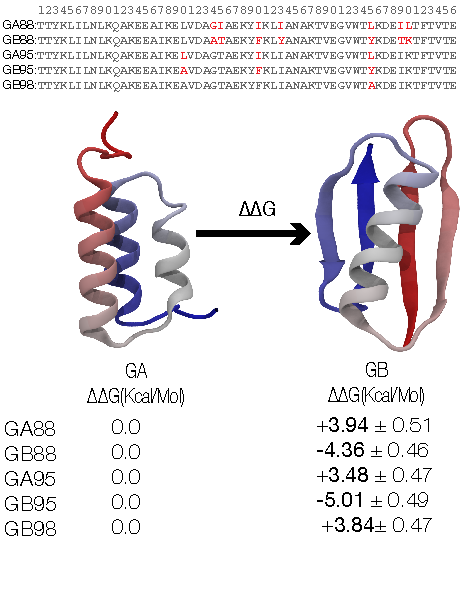
\includegraphics[width=3.5 in,height=4 in]{orban.pdf}
\label{fig:orban}
\caption{The confinement method correctly predicts the structural preferences of six chameleon
sequences. (A) The six sequences used in this study. (B) Each sequence adopts either a Protein
G-like fold (denoted GB) or a three-helix bundle fold (denoted GA). The relative free energies of
the two folds are reported for each sequence.}
\end{figure}

\begin{figure}
\includegraphics[width=6.5 in,height=5.4 in]{orban_full.pdf}
\label{fig:orban_full}
\caption{Orientation of residues of different sidechains in $4 \beta + \alpha$ and $3 \alpha$ form
A. Orientation of Hydrophobic residues Leu-5 and Leu-7.
B. Gln-11 has H-bond with Glu-15 in $3 \alpha$, which is absent in $4 \beta + \alpha$
C. Hydrophobic Ala-26
D. Hydrophobic Val-54.
E. Hydrophilic Glu-14.
F. The plot of free energy difference for GA95 and GB95 sequence. Positive peak stabilize $3 \alpha$ form and negative peak 
stabilize $4 \beta + \alpha$. 
G. Hydrophilic Glu-56 .
H. Orientation of Hydrophic Ile-49.
I. With GA95 sequence, Ile-49 have hydrophic interaction with both Leu-20 and Ile-30.
J. Larger Phe-30 in GB sequence, move towards the protein surface in $4 \beta + \alpha$.
K. Tyr-45 form H-bond with Asp-47 in $4 \beta + \alpha$.}  
\end{figure}

%\begin{table}
%\caption{The confinement method correctly reproduces the structural preferences of a series of
%designed peptides. Each sequence adopts either a Protein G-like fold ($4 \beta + \alpha$) or forms a
%helix bundle ($3 \alpha$).}
%\label{table:orban}
%\begin{center}
%\begin{tabular}{l l l}\hline
%Changes in & $\Delta G$ (kcal/mol)    & $\Delta G$ (kcal/mol)     \\
 %Sequences & ($3 \alpha$ fold)        & ($4 \beta + \alpha$ fold) \\ \hline
%GA95       & $0.000$                  & $2.901 \pm 0.475$         \\
%GB95       & $4.365 \pm 0.460$        & $0.000$                   \\
%GA88       & $0.000$                  & $ 3.941 \pm 0.517$        \\
%GB88       & $5.576 \pm 0.464$        & $0.000$                   \\
%GA98       &  &                           \\ \hline
%GB98       &                          &                           \\ \hline
%\end{tabular}
%\end{center}
%\end{table}


\subsection{The confinement method correctly identifies the most native-like predictions from a
subset of CASP predictions}

%\Alberto{Arijit: we need a global table of success, rather than individual tables. The simplest form
%    would have 3 columns: name of the PDB, number of structures tested, percent of success of
%    picking 1st model}

This method is particularly well suited to pick out the native/native like structure from misfolded or decoys. We have
tested this using different models from CASP (critical assessment of structure
prediction). CASP is a blind test in which different groups world wide apply their
methods to predict the 3D structure of proteins given their sequence. This is done with a strict 3
week limit on each target (3 day for servers) and each group is allowed to submit 5 possible
structures (ranked from best to worst). In our role as assessors during the CASP8 and CASP9 \cite{MacCallum2011}
competition we observed no correlation at all between the ordering of structures submited by the
groups and the real ranking compared to an experimental model \cite{Kryshtafovych2011}. The
consequences of this goes beyond
those five structures; the deeper meaning is that groups producing ensembles of structures are
generating structures that are better than the ones they submit, but they do not know about it. In
fact, when querrying different groups after the results were known, most groups agree that this is
the case. Beyond the CASP problem, this reflects on the modelers ability to correctly rank order
models in many different environments, such as structures for drug design leads or designing more
stable proteins or peptide mimetics such as peptoids. One of the main culprits of this lack of
accuracy is the fact that ranking is often done via a potential energy function, which in many cases
lacks an entropy component. Other initiatives including knowledge based potentials do use some sort
of free energy to rank order, but its accuracy is not enough. Our method provides a physics based
solution to this problem. We have tried two experiments centered on CASP. First we tried to rank
order some structures from the previous CASP9 experiment. We have tested different options for that purpose.
First, we rank order submitions from same group and then from different groups. Our second test was 
to check whether this method can do better quality assessment/metaprediction than the best group in that catagory in CASP9. 
In both methods, our ranking is determined as a free energy measure,
and it is compared with the ranking given by a geometrical comparison between native and submitted
models called GDT\_TS (Global distance test score \cite{Zemla2003}). 
GDT\_TS represents the average percentage of residues that are in close proximity in two
structures optimally superimposed using four different distance cutoffs (1, 2, 4 and 8 Å).

We have chosen the inital models on which to test the methods based on server groups that have
traditionally done good in past CASP events. There is a high correlation between the structures that
are chosen for this method and its predictive accuracy. In particular, when GDT\_TS scores are below
50, it is difficult for us to say anything about the models. Our approach is simple, for every
subset of structures we choose, we use the confinement method in a pairwise procedure, and then rank
the structures. In all cases, we have also calculated the free energy with respect to the native
structure to check the stability of the models.
However, this step is not needed if we just want to rank order.

\subsubsection{The confinement method can rank different models generated by the same methodology and distinguish the native structure}

The question that we want to answer here is whether we can rank models that have been generated with
the same methodology. In all cases, we have calculated the free energy
difference between the native structure and the submitted models as well. 
%Identifying the native state from a set of models is a very easy test, that most metapredictors
%already handle correctly, but it is also a first proof of principle. 
First we choose a protein BVU3908 from Bacteroides vulgatus whose PDB id and CASP target code are
2L01 and T0559 respectively. The native structure of this 69 residue protein was solved using NMR.
The best predictor group for this target was "BAKER-ROSETTASERVER".
We initially checked similarity between the models submitted by "BAKER-ROSETTASERVER" and discarded two of them from the 
analysis on the basis of being too similar to some of the other models. The GDT\_TS score and rmsd
values as shown in Figure~\ref{fig:T0559} indicate that model 1 was predicted correctly, 
whereas the order of model 3 and 5 was wrong. The main difference
between model 3 and the rest of the models is that the orientation of the first alpha helix of model
3 is \Alberto{opposite??}.
On the other hand, as shown in Figure~\ref{fig:T0559} the confine and release method not only can differentiate the native 
structure from the submitted models, the ranking also correlates perfectly with the GDT\_TS score.  

To further test the method we have taken the example of protein BT2368 from Bacteroides thetaiotaomicron. The PDB id of this 
74 amino acid residue protein is 2L02 and CASP target code is T0560. We have compared the free energy difference between 
the native structure and the two of the five submitted models from the group "Splicer". The remaining three models are discarded as 
again they are similar to the rest of the models. The comparison of GDT\_TS score as shown in 
Figure~\ref{fig:T0560} and published in the final CASP result is only for models with residues 3 to 66. In order to keep
consistency, we have also done our analysis with models and crystal structure consisting residues 3 to 66. As expected,
the native state is identified correctly, and the two other models are ranked in the correct order in accordance with the GDT\_TS score.   

\subsubsection{The confinement method can rank models generated by different methods}

Our next test was between models that are produced with different methodologies. We do this by
looking at some of the best CASP submissions from different research groups. 
For this purpose we have chosen the x-ray crystallographic structure of 
fas apoptosis inhibitory protein molecule whose pdb id and CASP target codes are 3MX7 and T0540 respectively.
This protein contain 90 amino acid residues with 8 beta strands. We have chosen best models from groups
"LTB" and "Mufold" for our analysis, which are labelled as Model 1 and Model 2 in Figure~\ref{fig:T0540}.
As presented in  Figure~\ref{fig:T0540} we found that this method is able to correctly order the models which matches
with the GDT\_TS score. 

\subsubsection{Per residue free energy calculation identifies the residues that are responsible for
differences between two conformations}

We used one of the CASP targets (pdb id=2KWY, casp id=T0569) to study the per residue contribution
between this NMR structure and the best CASP9 predicted model (from the 'Mufold' group, GDT\_TS=78).
Visualization upon superimposition of two structures reveals that
the difference between the two structure is at the region consist of residues 48 to 65, where model1 is much more disordered compare to the
native structure(see Figure~\ref{fig:T0569}). Other regions look similar for both the cases with of model1 is within 2.6 \AA backbone
rmsd value of the native structure. We found that, the confinement method can still differentiate between the native structure and 
the generated model. We have also calculated the per residue free energy with a aim that this can identify the residue which are responsible
for such free enerfy difference. The per residue free energy decomposition is shown in  Figure~\ref{fig:T0569_per_residue}(A). We indeed 
found that two hydrophobic residues Val-59 and Ile-61 are oriented towards the solvent in the protein 
surface in the generated model (Figure~\ref{fig:T0569_per_residue}(B). This the region, where there is a beta sheet in the original crystal structure, which is absent in the 
model. Interestinlgy, some regions are more stable in the generated model. A close inspection
reveals that 
the hydrophilic Glu in position 67 is completely exposed to the protein surface and solvent in the best model, whereas it is partially exposed in the 
crystal (Figure~\ref{fig:T0569_per_residue}(C)). The peak at position 76 is due to the H-bond between Lys-76 and Asp-11, 
which is absent in the original crystalographic structure (Figure~\ref{fig:T0569_per_residue}(D)). 
   
\subsubsection{Failures in the confinement method}

Despite the great success in most of the studied systems, we found a few failures, specially when
the GDT scores of the compared structures are
very close. We have found this for an engineered protein from Asr4154 protein (PDB ID: 2L09 and CASP Target T0538).
This protein contains 54 amino acid residues with three alpha helixes and two very short beta
strands. 
The model that is closest to the native structure was generated by the group PconsR with a GDT\_TS value of 96.23.
We have also considered one model from group "Shell" (GDT\_TS = 90.09) and "FOLDIT" (GDT\_TS = 86.32) for our analysis along with
the native crystal struture (RMSD values between 1.6 and 2.0\AA \Alberto{from native, right?all
atom? CA?}). The models from PconsR, Shell and FOLDIT are labelled as model 1, model 2 and model 3 
respectively in Figure~\ref{fig:T0538}. As seen in Figure~\ref{fig:T0538}, one can find that the 
model from PconsR has lowest free energy value, making it a more stable structure. Although ranking of the other models
remains consistent, model 1 is predicted to be more stable than the
crystal structure. To rationalize this, we have decomposed the total free energy into the per
residue components. The results show us that despite the small variation at the backbone level (as
shown by high GDT\_TS scores and low RMSDs), the sidechains are oriented in very different ways,
giving raise to large differences in the stabilization of certain residues.
In particular, some of the differences arise from different salt bridge patterns (Arg-32 with Glu-35
and Glu-28 with Lys-24
in crystal versus Arg-32 with Glu-28 in model 1) and certain flexible polar residues exposed to the
surface (Lys-24 in model 1, which has an entropic gain from not forming a salt bridge and is
stabilized by interactions with the solvent). This is summarized in Figure~\ref{fig:T0538compare}(A) 
Similar patterns arise in other places of the protein (see Figure ~\ref{fig:T0538compare}(B)), where
the salt bridge between Arg-26 and Glu-50 is absent in model 1 and is further \Alberto{stabilized?} by Phe-51
having a very different conformation that in the crystal structure.
All in all, this unexpected result just shows us that this method is sensitive to local interactions
such as those happening from side chain reorientation. At the same time, the results explained in
past sections showed that for larger changes the accuracy of the method is very high.

\subsubsection{What can we say about low resolution models?}

So far we have seen that the method is good at predicting preferences when the structures are not
very close to each other, how far from native can we go? In this section we want to explore what
happens when we use the method to describe low quality models. We use one of the CASP targets (pdb
id = 2KJX, CASP id = T0531) .
We mentioned earlier that our predictive abilities are greatly decreased with low model qualities. 
Comparing low qualitive models between themselves is not very informative,
    however, comparing all of them to a native/native like structure, allows to rank order this
structures. 
In order to test this hypothesis we performed another test with target T0531 of CASP9, in which we compared the crystal 
structure to five models from the MUFOLD server. Pdb id of this extracellular domain of the jumping translocation 
breakpoint protein is 2KJX and CASP target code is T0531.
Looking at Figure~\ref{fig:T0531} shows: 1.) native is correctly
identified as expected and 2.) Surprisingly there is a high level of correlation between the GDT
ranking and the free energy ranking for model 1 and model 3, the rest three structures with GDT\_TS score less than  35  are ordered
incorrectly. It is worth to note that models 2 and 3 have the same GDT and very different free
energies, meaning that the actual ordering could change a lot \cite{Perez2012}. It is encouraging that at least
the method can pick out the best model even though it is got a low GDT score: 44.  

%\subsubsection{Difficulty in CASP Experiments}

%It is often difficult to model CASP targets using the confinement and release method. There are many cases,
%where the sequence of a particular target is trimmed during actual result presentation. This is illustrated
%with the crystal structure of the leucine zipper domain of cGMP dependent protein kinase I (pdb id: 3NMD
%and CASP9 code: T0605) as shown in Figure~\ref{fig:T0605}. The actual CASP 9 target consisted of 72 amino acid residues, but
%as only 18-66 amino acid residues could be detected in actual crystal structure of this protein, the final result was trimmed 
%with respect to that crystal structure with 49 amino acid residues which consist of a single alpha helix. The amino acid residues 18 and 66 are shown in
%three models submitted by the group "Baker". It is important to note that blind prediction of model ranking on the basis of free energy can be hugely 
%affected in such scenario as the only major difference between those models are the trimmed parts, specially the region consisting residues 1-18.    


\subsubsection{Can the confinement method perform better quality assessment in protein structure prediction?}
A part of the CASP experiment is dedicated to the assessment of the quality of predicted models \cite{Kryshtafovych2011}. 
Most of the top performing groups in this category use consensus approaches for quality assessment \cite{Wang2011}.
A review of CASP9 quality assessment also pointed out that the methods which are based on clustering
techniques perform
much better compared to those methods which are based on analysis of individual models \cite{Kryshtafovych2011}. 
In this background we try to answer, whether the confinement method can do better quality assessment
compared to the best performing
group (MUFOLD-WQA) in this catagory. In CASP9, the overall reliability of models in quality assessment (QA) was accepted in a mode known as
QMODE 1. Here, predictors were asked to score each model on a scale from 0 to 1, with higher values corresponding to better models \cite{Kryshtafovych2011}. 
We have again picked up the CASP taget T0538 to answer this question. We have chosen Model 3 submitted by PconsR (GDT\_TS = 96, QMODE 1 = 0.5434) 
and model 5 from the MULTICOM-NOVEL ( GDT\_TS = 83, QMODE 1 = 0.5865). Both are server predicted models and they were further used for quality assessment 
by the group MUFOLD-WQA \cite{Wang2011}. It is important to note that the model from PconsR was the most accurate predicted model for this 
target and the model from MULTICOM-NOVEL was predicted as best by the quality assessment experiments of MUFOLD-WQA. Also, 
the QMODE 1 value presented here is from the group MUFOLD-WQA. 
Our free energy analysis predict that the model from Pconsr is indeed better than the model from 
MULTICOM-NOVEL $(\Delta \Delta G (Model\_Pconsr - Model\_MULTICOM-NOVEL = -3.9 Kcal/Mol)$, which   
matches well with the GDT\_TS score. On the other hand the MUFOLD-WQA predicted the ranking in the reverse order. 

We have also carried out a similar type of analysis for the case of Target 560 from the CASP9 experiment. For that 
we have chosen the model 1 from the group PconsR (GDT\_TS = 94, QMODE 1 = 0.5178), Bilab\-Enable (GDT\_TS = 87, QMODE 1 = 0.5344) 
and Multicom\_Refine (GDT\_TS = 74, QMODE 1 = 0.4770). If, one wants to rank order with respect to the GDT\_TS values, the model from 
PconsR is the best predicted model, but according to the QA assessment by MUFOLD-WQA, the model from Bilab-Enable was found to be best predicted model. 
All the QMODE 1 values are from MUFOLD\-WQA. In CASP 9, the sequence of 74 residues were given to predict the structure and for 
quality assessment, whereas during GDT\_TS analysis only residues 3-66 were considered. When we considered the full 74 amino acid 
residues, the free energy calculated were $(\Delta \Delta G (Model\_Pconsr - Model\_Bilab\-Enable = 3.3 Kcal/Mol)$ and 
$(\Delta \Delta G (Model\_Pconsr - Model\_Multicom\_Refine = -30.0 Kcal/Mol)$ \Alberto{-30 sounds
huge!} which 
support the QA assessment by MUFOLD-WQA. On the other hand, if we calculate the same free energy with the trimmed version of the protein 
(with residues 3-66), the values of the free energy difference become -1.7 and -31.1 Kcal/Mol respectively, which support the GDT\_TS score. 
The summary of this whole observation is presented in Table~\ref{table:560QA}.
There is no doubt that the consensus approach can predict the model quality in a faster manner. But
we expect that the confinement
method can predict the model quality in a relatively expensive but much more accurate way.

\begin{table}
\label{table:560QA}
\begin{center}
\begin{tabular}{| l | l | l | l | l |}
\hline
Model            &  $\Delta \Delta G$ (1-74)  & $\Delta \Delta G$ (3-66) &    GDT\_TS    & QMODE 1  \\ \hline
PconsR           &         0.0                &      0.0                 &    94         &  0.5178   \\ \hline
Bilab\-Enable     &        -3.3                &      1.7                 &    87         &  0.5344   \\ \hline
Multicom\_Refine &        30.0                &     31.1                 &    74         &  0.4770   \\ \hline
\end{tabular}
\end{center}
\caption{Comparison of quality assessment by the group MUFOLD\-WQA and the confinement method of the CASP9 target 560 (pdb id: 2L02). 
The GDT\_TS score obtained from CASP9 website, was based on the trimmed model containing residue 3-66, whereas, the QMODE 1 values are from
quality assessment by the group MUFOLD\-WQA and based on residues 1-74.}
\end{table}  


\section{Conclusion}


\Alberto{The last 50 years represent our effort to understand what the native state of a protein
    looks like by using theoretical methods. Experimental evidence coming from NMR and x-ray
    cristallography remain so far the only real ways to solve the structure of the native state.
    However, this methods are expensive and slow. Theoretical methods on the other hand are cheaper,
    but despite improvement still have a long way to go. Often this computational pipelines produce
    ensembles of diverse structures and identifying which structure is more native like is still a
    problem. Here we have shown how the application of the confinement method can help identify
    native like states. The high success rate balances with the computational expense. However, with
    GPU technology and the rate at which computers improve, this computational expense is becoming
less of a bottle neck.}
\Alberto{I don't agree with some of the points here, but I think I covered what you meant in the
previous paragraph}
In the recent past there have been a number of studies directed towards understanding protein 
structure using theoretical tools. Experimentally, it is relatively easy to identify the native structure from the data obtained 
from x-ray crystallography or NMR. On the other hand using theoretical tools it is often difficult to identify the native structure 
using both physics based methods and knowledge based method. In order to rank structure from the available data, some groups use 
clustering algorithms and the structure of the
most populated cluster is picked out as the most probable structure. However, it may happen that the structure may be trapped and 
spend most of its time in a kinetic trap ***kinetic traps in MD,not other methods, local
minima***, which may give a wrong interpretation of the clustering result. On the other hand, some groups
also depend on potential energy functions to pick out their best structure, lacking an entropic
component. In this work we attempted to identify the native/native like protein strcuture from the decoy using free energy as a scale.
We have used the previously developed confinement method, applying it to larger systems.

We found that in majority of cases, the native structure is always the most stable and we can rank
protein structures upto 100 amino 
acid residues long. This method works very well if at least one of the strcuture in the decoy set
has high quality. The main advantage of this method is 
that it does not require any reaction coordinate. Thus one can calculate the free energy difference between two very different conformations. 
An interesting application from this method that we have exploited is the partition of free energies
on a per residue basis.
 Although, it is an approximate partition, it gives important insight regarding the conformational 
preferences of a particular residue. The use of this decomposition in understanding the effect of a
small number of aminoacids in our test chamaleon sequences allows us to think that in the future,
this method may be used for protein design. 
The method can be also give wrong result if all the models in the decoy are very poor. It may also be difficult to rank structures if 
all the structures are very very close to the native structure. But that does not matter at all as our main aim is to differentiate
between the good and the bad structure. In this article we have extensively tested this method using examples from CASP experiment.
This method can be computationally expensive in actual CASP experiment if one want rank hundreds of submitted models in CASP 
experiments. However, in real life experiment with a particular target, we expect this method can give accurate result. The important 
fact about confinement method is that all the part of the calculation can be done independently. 
There is another big bottlenecks in this calculation. This has to do with the amount of
simulations that have to be performed to confine the ensemble of conformations close to a microstate
into a single microstate. We have tackled this issue by using GPU (Graphical Processing Unit) technology as opposed to the classical
CPUs, which gives us a two order of magnitude boost in computational efficiency.
For example, we have mostly carried out our calculation with Amber program \cite{Case2005} in GPU computer. With a avarage 56 residue 
we found that it take only 4 hour to complete 20 ns of the confinement step. So, with available computer power this method will 
be easy to use for real problems. 
%There is another issue, which is normal mode
%analysis calculations are Oh(N**3) and require large amounts of memory, effectively limiting the
%size of the systems under study. In most cases quasiharmonic analysis.   
 
This method can be further used for calculating free energy due to very large conformational change. Another application may be
for the case of ligand binding. It can also be used to distinguish the most stable structure during protein design. Decompition of 
total free energy into the per residue component help identifying residues that give stability to a particular conformation. 
Another, important application may be to study the protein folding kinetics, specially to study the phi value analysis.            


\section{Method}

The confinement method has been described in details in ref. by Tyka et.al. \cite{Tyka2006} and 
Cecchini et. al. \cite{Cecchini2009}. The basic approach of the confinement approach is the same in both
these papers. However, there are some technical differences. Here we briefly describe the procedure
to compute free energy $\Delta G_{AB}$ between two conformations A and B of a protein. The basic
idea to compute the free energy between conformations A and B is to perform a thermodynamic cycle: 

\begin{enumerate}

\item  Minimization of A and B. These minimized conformations (A* and B*) 
       are the reference conformation of that state. During this minimization the backbone is kept
       restrained to the original position to avoid large conformational changes.

   \item  The free energy of confining the ensemble (A or B) to a microstate (A* or B*) is
       calculated. This is done by gradually applying larger and larger
       harmonic restraints on all the atoms of the biomolecule. This is done by running 21 molecular dynamics simulation 
       (20 ns long each), where the harmonic restraint force constant was scaled from 0.00005
       \Alberto{units??}
       (mostly free) to 81.92 (frozen in one microstate). In this final restrained state, the
       rotational contribution to the free energy is frozen out
       and the only remaining contribution is the vibrational part. The free energy for this step is
       estimated from the fluctuations around
       the reference structure using a numerical
       approach developed by Tyka et. al. \cite{Tyka2006}. The confinement free energy calculated in
       this way is recorded as 
       $\Delta G_{A,A*}$ and $\Delta G_{B,B*}$ as shown in Figure~\ref{fig:method}.     

\item  Finally the thermodynamic cycle is closed by calculating the free energy between the final
       restrained state A* and B* using normal mode analysis or quasiharmonic analysis. The free energy calculated in 
       this way is shown as $\Delta G_{A*,B*}$ in Figure~\ref{fig:method}.

\item  The full free energy, $\Delta G_{A,B}$ between the two state A and B is calculated using the equation 
       $\Delta G_{A,B}$ = $\Delta G_{A,A*}$ - $\Delta G_{B,B*}$ + $\Delta G_{A*,B*}$  

\end{enumerate}

 All calculations where performed with the amber 11 suit of programs in combination with ff99SB and GB/SA implicit solvent. Interestingly, we extend the
method for calculation of per residue free energy in an approximate way. For this purpose, the confinement energy, 
$\Delta G_{A,A*}$ and $\Delta G_{B,B*}$ of each residue is calculated in the usual numerical way as described above. The
internal energy of each residue is calculated using the decomp module of amber from the final restrained trajectory. We 
call this method approximate as we ignore the contribution from the normal mode or quasiharmonic analysis. 
However, this contrbution to the total free energy is much smaller (less than $1.0
Kcal/Mol$\Alberto{that sounds huge, i would say what percent of error we stimate, I think it was
lower than 1kcal/mol}), which allow us to 
study the mechanistic details of conformational preference of each residue.      

%There are two big bottlenecks in this calculation. The first has to do with the amount of
%simulations that have to be performed to confine the ensemble of conformations close to a microstate
%into a single microstate, the second bottleneck has to do with the size of the system in the normal
%mode calculation. We have tackled the first issue by using GPU (Graphical Processing Unit) technology as opposed to the classical
%CPUs, which gives us a two order of magnitude boost in computational efficiency. Normal mode
%analysis calculations are Oh(N**3) and require large amounts of memory, effectively limiting the
%size of the systems under study. Where as this can be overcome by larger memory machines, these are
%often not available, and so we propose an alternative by using quasiharmonic analysis. This is still
%an Oh(N**3) problem, but we now the motions of atoms are already determined in trajectories, and so
%we can choose to do quasiharmonic analysis excluding hydrogens, which will reduce the number of
%atoms N to almost N/2. This means that we can use this method for systems twice as large.


\begin{figure}
\begin{center}
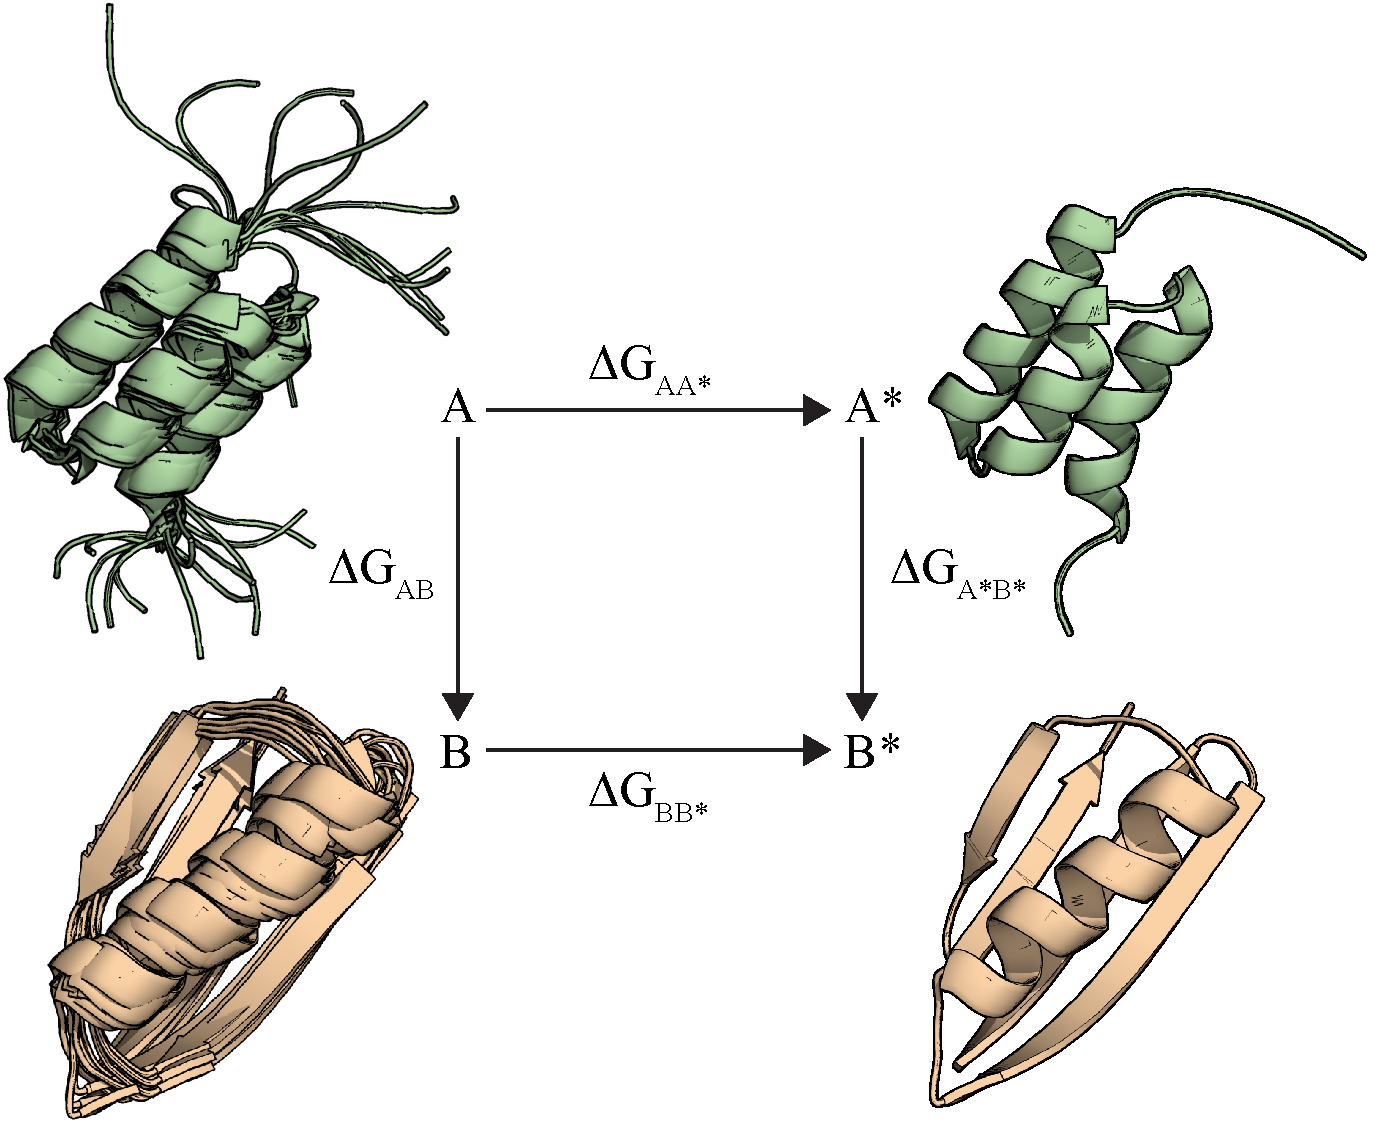
\includegraphics[width=3.5 in,height=3.5 in]{method.pdf}
\end{center}
\caption{Graphical representation of the thermodynamic cycle involving confinement method.}
\label{fig:method}
\end{figure}

%\begin{figure}
%\begin{center}
%\includegraphics[width=3.5 in,height=3.0 in]{G95.pdf}
%\end{center}
%\caption{Two protein with 95 \% similar sequence but different folds}
%\label{fig:G95}
%\end{figure}

\begin{figure}
\begin{center}
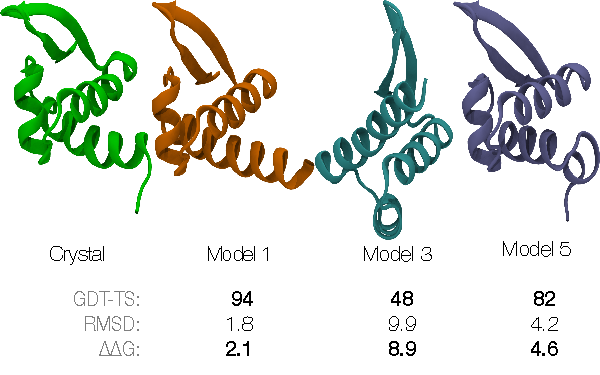
\includegraphics[width=3.8 in,height=3.0 in]{T0559.pdf}
\end{center}
\caption{The native and three submitted model structure, along with their GDT\_TS, RMSD and relative Free energy values 
of protein BVU3908 from Bacteroides vulgatus (PDB id: 2L01 and CASP code: T0559).}
\label{fig:T0559}
\end{figure}

\begin{figure}
\begin{center}
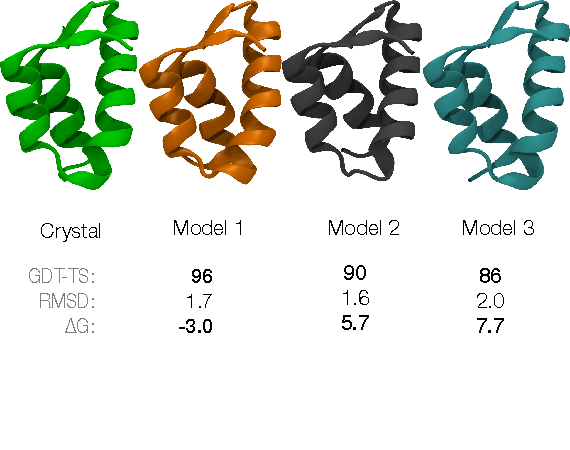
\includegraphics[width=3.8 in,height=3.0 in]{T0538.pdf}
\end{center}
\caption{The native and three model structure of engineered protein from Asr4154 protein (PDB ID: 2L09 and CASP code:T0538). The model 1,2 and 3 are
from the group PconsR, Shell and FOLDIT respectively.}
\label{fig:T0538}
\end{figure}

\begin{figure}
\begin{center}
\includegraphics[width=4.9 in,height=4.0 in]{Target_538_compare.pdf}
\end{center}
\caption{Difference of the sidechain orientation between model 1 and crystallographic structure in Target-538.
A. The salt bridge between Glu-35 and Arg-32 in crystal structure. In model 1, this is compensated by H-bonding between 
Arg-32 and Glu-28. There is another salt bridge between Glu-28 and Lys-24.
B. Salt bridge between Arg-26 and Glu-50 in crystal structure. Orientation of Phe-51 is different in crystal than in model1.}
\label{fig:T0538compare}
\end{figure}


\begin{figure}
\begin{center}
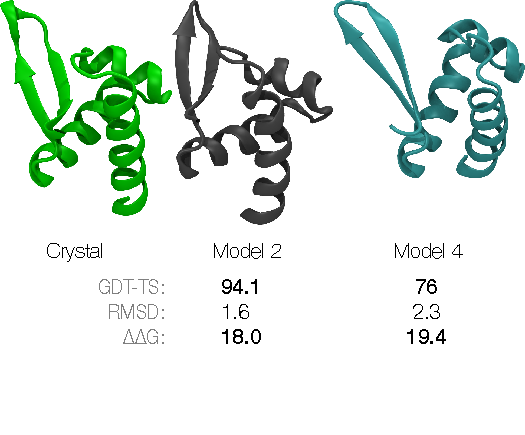
\includegraphics[width=3.5 in,height=3.0 in]{T0560.pdf}
\end{center}
\caption{Native and two model structure of protein BT2368 from Bacteroides thetaiotaomicron (pdb id: 2L02 and CASP code: T0560). The two models
were from the group "Splicer".}
\label{fig:T0560}
\end{figure}

\begin{figure}
\begin{center}
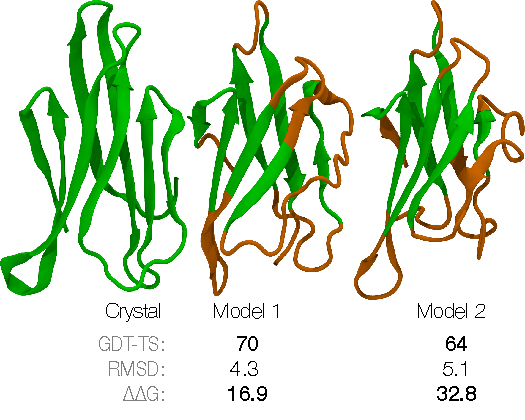
\includegraphics[width=3.5 in,height=3.0 in]{T0540.pdf}
\end{center}
\caption{X-ray crystallographic structure and two submitted models of fas apoptosis inhibitory protein (pdb id: 3MX7 and CASP code: T0540). 
Model 1 and Model 2 in this analysis were submitted by the group LTB and MUFOLD respectively.}
\label{fig:T0540}
\end{figure}

\begin{figure}
\begin{center}
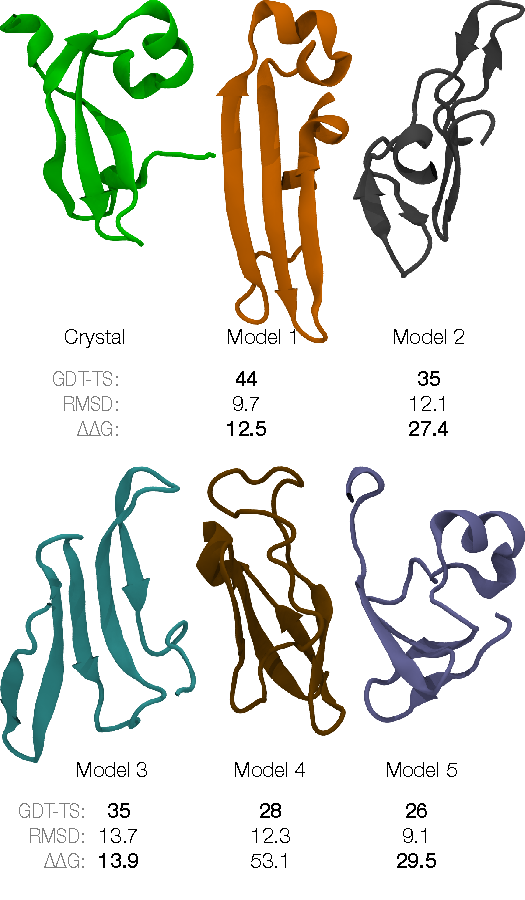
\includegraphics[width=3.5 in,height=5.7 in]{T0531.pdf}
\end{center}
\caption{The native structure and 5 models of extracellular domain of the jumping translocation
breakpoint protein (pdb id: 2KJX and the CASP code: T0531).}
\label{fig:T0531}
\end{figure}

\begin{figure}
\begin{center}
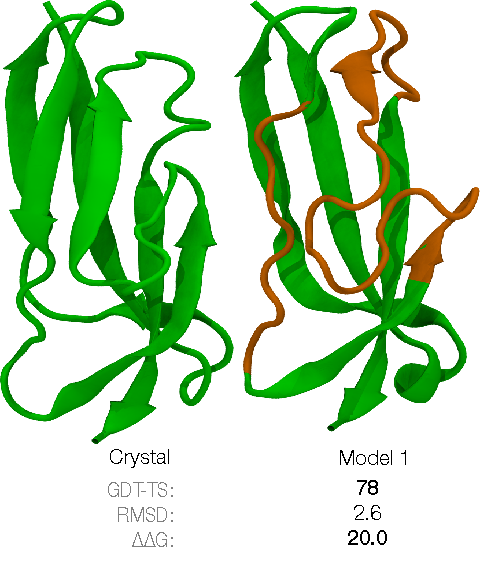
\includegraphics[width=3.2 in,height=3.8 in]{T0569.pdf}
\end{center}
\caption{Native and best model structure of a domain of adhesion exoprotein from Pediococcus pentosaceus (pdb id: 2KWY and CASP code: T0569).
The best model was from the group "Mufold".}
\label{fig:T0569}
\end{figure}

\begin{figure}
\begin{center}
\includegraphics[width=5 in,height=4 in]{Target_569_per_residue.pdf}
\end{center}
\caption{A. Plot of per residue free energy difference between the model and the crystal structure of Traget 569 (pdb id: 2KWY) of CASP9.
B. In model 1, the beta sheet containing Val-59 and Ile-61 is disordered. These hydrophobic residues are exposed to the solvent.
C. Glu-67 is partially exposed to the solvent in crystal and it is fully exposed in model 1.
D. There is a H-bond between Lys-76 and Asp-11 in model 1, which is absent in the crystallaographic structure.}
\label{fig:T0569_per_residue}
\end{figure}


%\begin{figure}
%\begin{center}
%\includegraphics[width=12cm,height=10cm]{T0605.pdf}
%\end{center}
%\caption{ Three models of the leucine zipper domain of cGMP dependent protein
%kinase I (original pdb id: 3NMD and CASP target: T0605). The original target sequence of this protein was 72 residues.
%However only residues 3 to 66 is only kept during result announcement as that part can be found from crystallographic analysis. The
%region 3 to 66 are almost identical in all the 3 models  }
%\label{fig:T0605}
%\end{figure}


\begin{thebibliography}{99}

\bibitem{Meirovitch2007}
Meirovitch, H. Recent developments in methodologies for calculating the entropy and free energy of biological systems by computer simulation.
Current Opinion in Structural Biology, 2007, 17, 181-186.

\bibitem{Chipot2007}
Chipot, C.; Shell, M.S.; Pohorille, A. Introduction, in Chipot, C., Pohorille, A., editors. Free Energy
Calculations: Theory and Applications in Chemistry and Biology. Springer Series in Chemical
Physics, vol. 86. Berlin and Heidelberg: Springer; 2007, p. 1–32.

\bibitem{Jorgensen2004}
Jorgensen, W.L. The many roles of computation in drug discovery, Science 2004, 303, 1813–8.

\bibitem{Gilson2007}
Gilson, M.K.; Zhou, H.X. Calculation of protein-ligand binding affinities. Annu Rev Biophys Biomol Struct. (2007) 36, 21-42.

\bibitem{Torrie1977}
Torrie, G. M.; Valleau, J. P. iNonphysical sampling distributions in Monte Carlo free-energy estimation: Umbrella sampling 
(1977) J. Comput. Phys. 23, 187

\bibitem{Tironi1994}
Tironi, I.G.; van Gunsteren, W.F. A molecular-dynamics simulation study of chloroform. Mol. Phys. (1994) 83, 381-403.

\bibitem{Dill1997}
Dill, K.A.; H.S. Chan.  From Levinthal to Pathways to Funnels:  The "New View" of Protein Folding Kinetics.  Nature Structural Biology 4, 10-19 (1997)

\bibitem{Dill2008}
Dill, K.A.; Ozkan, S.B.; Shell, M.S.; Weikl, T.R. The protein folding problem. Annual Review of Biophysics (2008), 37, 289-316.

\bibitem{Anfinsen1973}
Anfinsen. C.B. Principles that Govern the Folding of Protein Chains. Science (1973) 181, 223-230.

\bibitem{Christ2007}
Christ, C.D.; van Gunsteren, W.F. Enveloping distribution sampling: A method to calculate free energy differences from a single simulation,
J. Chem. Phys. (2007), 126, 184110.

\bibitem{Ytreberg2006}
Ytreberg, F.; Zuckerman, D. Simple estimation of absolute free energies for biomolecules. J. Chem. Phys. 2006, 124, 104105.

\bibitem{Park2008}
Park, S.; Lau, A.; Roux, B. Computing conformational free energy by deactivated morphing. J. Chem. Phys. 2008, 129, 134102

\bibitem{Zheng2008}
Zheng, L.; Chen, M.; Yang, W. Random walk in orthogonal space to achieve efficient free-energy simulation of complex systems, Proc. Natl. Acad. Sci. 2008, 105 (51), 20227.

\bibitem{Tyka2006}
Tyka, M.; Clarke, A.; Sessions, R. An Efficient, Path-Independent Method for Free-Energy Calculations. J.Phys.Chem. B 2006, 110, 17212-17220.

\bibitem{Cecchini2009}
Cecchini, M., Krivov, S.V., Spichty, M., Karplus, M. Calculation of free-energy differences by confinement simulations. Application to peptide conformers. 
J. Phys. Chem. B 113, p. 9728-9740 (2009).

\bibitem{Strajbl2000}
Strajbl, M.; Sham, Y.Y.; Villà, J.; Chu, Z.-T.; Warshel, A. Calculations of Activation Entropies of Chemical Reactions 
in Solution. (2000) 104, 4578-4584.  

\bibitem{Krivov2004} 
Krivov, S.; Karplus, M. Hidden complexity of free energy surfaces for peptide (protein) folding Proc. Natl. Acad. Sci. U.S.A. 2004, 101, (41), 14766.

\bibitem{Alexander2007}
Alexander, P.A.; He, Y.; Chen, Y.; Orban, J. Bryan, P. The design and characterization of two proteins with $88 \%$ sequence identity but different 
structure and function. Proc. Natl. Acad. Sci. 2007, 104 (29), 11963-11968.

\bibitem{He2008}
He, Y.; Chen, Y.; Alexander, P.A.; Orban, J. NMR structures of two designed proteins with high sequence identity but different fold and function. Proc. Natl. Acad. Sci. 2008, 105 (38), 14412-14417.

\bibitem{Alexander2009}
Alexander, P.A.; He, Y.; Chen, Y.; Orban, J. Bryan, P. A minimal sequence code for switching protein structure and function. Proc. Natl. Acad. Sci. 2009, 106(50), 21149-21154.

\bibitem{Shortle20009}
Shortle, D. One sequence plus one mutation equals two folds. Proc. Natl. Acad. Sci. 2009, 106(50), 21011-21012. 

\bibitem{Sheffler2009}
Sheffler, W.; Baker, D. RosettaHoles: Rapid assessment of protein core packing for structure prediction, refinement, design, and validation. Protein Science. 2009, 18(1), 229-239.


\bibitem{MacCallum2011}
MacCallum, J.; Perez, A.; Schnieders, MJ.; Hua, L.; Jacobson, M.P.; Dill, K.A. Assessment of protein structure refinement 
in CASP9. Proteins, 2011, 79, 74-90.

\bibitem{Kryshtafovych2011}
Kryshtafovych, A.; Fidelis, K; and Tramontano, A. Evaluation of model quality predictions in CASP9. Proteins, 2011, 79, 91–106

\bibitem{Zemla2003}
Zemla, A. LGA: a method for finding 3D similarities in protein structures. Nucleic Acids Res 2003, 31, 3370–3374.


\bibitem{Perez2012}
Perez, A.; Yang, Z.; Bahar, I.; Dill, K.A.; MacCallum, J.L.; FlexE: Using Elastic Network Models to Compare Models of Protein Structure. J. Chem. Theory Comput., 2012, 8, 3985-3991. 

\bibitem{Wang2011}
Wang, Q.; Vantasin, K.; Xu, D.; Shang, Y. MUFOLD-WQA: A new selective consensus method for quality assessment in protein structure prediction. 
Proteins, 2011, 79: 185–195. 

\bibitem{Case2005}
Case, D.A.; Cheatham, III, T.E.; Darden, T.; Gohlke, Luo, H.R.; Merz, Jr., K.M.;  Onufriev, A; Simmerling, C.; 
Wang, B.; R. Woods, R. The Amber biomolecular simulation programs. J. Computat. Chem. (20005) 26, 1668-1688.



\end{thebibliography}

\end{document}

